\documentclass{article}
%\usepackage[a4paper, total={6in, 8in}]{geometry}
\usepackage{geometry}
 \geometry{
 a4paper,
 total={210mm,297mm},
 left=20mm,
 right=20mm,
 top=-2mm,
 bottom=2mm,
 }
%\usepackage[margin=0.5in]{geometry}
\usepackage[utf8]{inputenc}
\usepackage{fourier} 
\usepackage{array}
\usepackage{makecell}
\renewcommand\theadalign{bc}
\renewcommand\theadfont{\bfseries}
\renewcommand\theadgape{\Gape[4pt]}
\renewcommand\cellgape{\Gape[4pt]}
\usepackage{amsmath,amssymb}
\usepackage{ifpdf}
\usepackage{fixltx2e}
%\usepackage{cite}
\usepackage{algorithm}
\usepackage{algorithmic}
\usepackage{array}
\usepackage{mdwmath}
\usepackage{pdfpages}
\usepackage{mdwtab}
\usepackage{eqparbox}
\usepackage{cite}
%\onecolumn
%\input{psfig}
\usepackage{color}
\usepackage{graphicx}
\setlength{\textheight}{23.5cm} \setlength{\topmargin}{-1.05cm}
\setlength{\textwidth}{6.5in} \setlength{\oddsidemargin}{-0.5cm}
\renewcommand{\baselinestretch}{1}
\pagenumbering{arabic}
\usepackage{ragged2e}
\usepackage[utf8]{inputenc}
\documentclass{article}
\usepackage[utf8]{inputenc}
\usepackage[english]{babel}
\usepackage[utf8]{inputenc}
\usepackage{amsmath}
\usepackage{array}
\usepackage{graphicx}
\usepackage{multirow}
\usepackage{optidef}
\usepackage[dvipsnames]{xcolor}
\renewcommand{\baselinestretch}{1.5}

\begin{document}

\textbf{
\begin{center}
{
\large{School of Engineering and Applied Science (SEAS), Ahmedabad University}\vspace{4mm}
}
\end{center}
%
\begin{center}
\large{B.Tech (ICT) Semester VI / M.tech / PhD: Machine Learning (CSE 523) }\\ \vspace{3mm}
\end{center}
}
\begin{itemize}
\item Group No : 21(Climate Changes and Environment 8)
\item Name (Roll No) :  Group Members

\begin{enumerate}
    \item Vishal Saha (AU 1741004)
    \item Rushil Shah (AU 1741009)
    \item Muskan Matwani (AU 1741027)
    \item Mohit Vaswani (AU 1741039)
\end{enumerate}\item Project Title: Air Quality Index Prediction

\item Project Area: Climate Changes and Environment 

\end{itemize} 

\section{Introduction}
  
\subsection{\color{brown} Background}

\begin{itemize}
     Air pollution is one of the major issue for mankind. It is also a main determinant of human health. Dealing with air pollution is even more challenging for the world in current times.Air pollution has been increasing a lot after industrial revolution.Rapid growth and improved lifestyle has led to an increase in air pollution considerably. It is one of the major concerns for the developing countries like India which is considered as one of the most polluted countries in the world. Developing countries like India, use fossil fuels for domestic and industrial purposes, incomplete combustion of these fuels result into emission of PM2.5, SO2 , RSPM etc. into air and pollutes the air. As a result of these air pollutants, there has been a huge increase in the level of global warming and irregular changes in climate. Hence, Precise air quality prediction and appropriate action plans to reduce air pollution, is our prime goal. Numerous machine learning techniques have been adopted that overcome these limitations and help us predict the air quality accurately. 
\end{itemize} 
\subsection{\color{brown} Literature Review}  

\begin{itemize}
In the last few decades, many machine learning techniques
have been proposed for analyzing and solving air pollution prediction problems. \\ \\
Many Researchers have tried to predict the quality of air using classification techniques. 
Athanasiadis et al. used s-fuzzy lattice neurocomputing classifier to classify O\textsubscript{3} concentrations into classes: [low, mid, and high] using meteorological features and some
pollutants : SO\textsubscript{2}, NO, NO\textsubscript{2}, and so on\textsuperscript{\cite{ref8}}. Kurt and Oktay used neural network model and predicted daily Air quality value by classifying it into categories using concentration values of SO2, CO, and PM10\textsuperscript{\cite{ref9}}. The drawback of converting regression problems into classification is that it ignores the magnitude of numeric data and produces discretized output (class label) losing the resolution that can be achieved using numeric data.\\ \\
Dan Wei used Naive Bayes classification and support vector machine to predict air quality in Beijing city\textsuperscript{\cite{ref10}}.
José Juan Carbajal et al. used fuzzy inference model to perform parameter classification using a reasoning process and integrating them into an air quality index\textsuperscript{\cite{ref11}}.
Shaban et al. created a wireless system to monitor and predict air quality to identify highly polluted area in a given city using support vector machines, M5P model trees, and artificial neural networks (ANN)\textsuperscript{\cite{ref14}}. Varun Jain et al. in their work "Scalable measurement of air pollution using COTS IoT devices" created a system to predict air quality by considering traffic conditions and the available greenery ,data is collected when users take a trip\textsuperscript{\cite{ref15}} this approach ignores the contribution of pollutants that degrade air quality and just focuses on the greenery present in the surrounding.So in the areas with sufficient amount of greenery and large Sulfur dioxide, Nitrogen Dioxide etc. pollutants emitting activities the Air Quality predicted would belong to healthy category which would be wrong result. MdNazmulHoq et al. in their work “Prediction of possible asthma attack from air pollutants: towards a high density air pollution map for smart cities to improve living” created a mobile application to predict the asthma attack on highly populated cities\textsuperscript{\cite{ref16}}.\\ \\
Dong et al. \textsuperscript{\cite{ref12}} used hidden semi markov
model while Thomas and Jacko \textsuperscript{\cite{ref13}} used basic regression and neural network to predict concentration of  PM\textsubscript{2 .5} in air.
Aditya C. R et al. used logistic regression is used to detect whether a data sample is either polluted or not polluted and used autoregression used to predict future values of PM\textsubscript{2.5} based on the previous PM\textsubscript{2.5} readings and thus they predict air quality\textsuperscript{\cite{ref17}}.
C. A. Keller et al.
proposed machine learning techniques for predicting the concentration of ozone in different countries. They used sparse sampling,
randomized matrix decompositions to
reduce the dimensionality of the data. They have used random forest regression technique for predicting O3 for the next 10 days\textsuperscript{\cite{ref22}}.
A. Ben Ishak et al. studied Ozone concentration at Tunisia. They have used three monitoring stations
for measuring ozone concentration and used Random forest
and Support vector Regression for future prediction. 
They have concluded that Random Forest performs better as an estimator to predict ozone concentration\textsuperscript{\cite{ref24 }}.This approach of taking only subset of the pollutants that contribute in deteriorating the air quality, into account while predicting air quality ignores the effect of other pollutants that contribute in degrading the air quality.In our model we calculate the AQI using EPA method considering the pollutants that have significant contribution in deciding the Air Quality.\\ \\

R. W. Gore et al. studied Air Quality Index and its effect on health.They used Decision tree
and Naive Bayes for classification.Their results showed that decision tree performs with approximately 92\% accuracy.The drawback with this implementation was that the data-set they used was limited and decision tree was unable to perform well on continuous values.
Asgari et al. have studied the urban Air pollution and
recorded them according to geographical areas. They have discovered the data of Tehran from 2009 to 2013 using Apache Spark. They have compared the prediction performance of Naive Bayes algorithm and Logistic Regression . They have concluded that the method of Naive Bayes to predict data produces more accurate results as compared to other machine learning
algorithms for classifying the priori known classes of air
quality. This implementation gives good performance in terms of Apache
Spark processing time but the machine learning algorithm used are
not logical for real-time time series prediction\textsuperscript{\cite{ref26}}.
C. Yan et al. in their work "Predictive
mapping of urban air pollution using Apache Spark on a Hadoop cluster." trained their model with meteorological parameters and then they trained their model by considering air pollutants into account.They claim that this implementation has made the system performance better in terms of accuracy.The drawback of this implementation is that they had considered only single stations and few hours data and due to this small size data-set their model faces the issue of overfitting. \textsuperscript{\cite{ref27}}. 

\\ 
  \end{itemize}  
\subsection{\color{brown} Related Work} 
  \begin{itemize}  
    \item Machine learning calculations and figurative power to predict the future, hence it has found its application in almost everywhere. Air Quality prediction problem is solved by many researchers using different algorithms. The main complication with Air Quality Index prediction is that,there are many factors to be considered. Some of the research works are closely related with our prime goal. For instance research work "Applying Machine learning Techniques in Air Quality Prediction" by Elias Kalapanidas and Nikolaos Avouris\textsuperscript{\cite{ref18}}, attempts to solve the same problem using Decision Tree and Naive Bayes Algorithm. The shortcomings of these methodology is, Decision tree is not a good classifier for time series.They also tried to approach this problem with a limited amount of data set, which increases the chances of over-fitting. Another research work "Forecasting Ozone concentration in smart city using deep learning" by Osama A. Ghoneim, Doreswamy, B. R. Manjunatha\textsuperscript{\cite{ref19}} . They have compared Support Vector Machine and NN machine learning Algorithms. The Short-coming of this research work is that they have considered only one feature to solve this complex problem. Another research work "A Machine Learning Approach for Air Quality Prediction: Model Regularization and Optimization" by Dixian Zhu , Changjie Cai , Tianbao Yang and Xun Zhou\textsuperscript{\cite{ref20}}.In this research work authors use ozone, SO2 and PM 2.5 for  AQI prediction. They also use regularization and optimization to predict future pollutant values. They have used linear regression to serve the purpose. The limitation of this research work is lack of generality. As they have developed model using data collected by only two data-stations.
    \item The Research work "Comparative Analysis of Machine Learning Techniques for Predicting Air Quality in Smart Cities" by Saba Ameer and other co-authors\textsuperscript{\cite{ref21}}. In this research work the authors have considered data-set of four Chinese cities, namely 'Beijing','Shanghai','Shenyang City','Guangzhou City' and 'Chengdu City'.The authors have considered different regression techniques, compared them and evaluated them based on Mean Absolute Error (MAE) and Root Mean Square Error (RMSE). Regression techniques such as Decision Tree Regression, Random Forest Regression, Gradient boosting Regression and Artificial Neural Networked Multi-layer Perception Regression were used to serve this complex problem. Decision tree regression was used to develop a predictive model with the help of simple decision rules. The random forest ensures that every tree in the ensemble is generated from a sample with replacement (bootstrapping) from the training set\textsuperscript{\cite{ref22}}.  Gradient boosting Regression was used for a better generalization of arbitrary differentiable loss function. Furthermore they have concluded that random forest regression technique performs best among all of the regression techniques taken into consideration.
    


\subsection{\color{brown} Motivation}
Air pollution is one of the main detriments to human health.
According to World Health Organization, 7 million people are
at health risk due to air pollution. It is a leading risk factor
for majority of health problems like asthma, skin infections,
heart issues, throat and eye diseases, bronchitis, lungs cancer
and respiratory system’s diseases. Besides the health problems
related to air pollution, it also poses a serious threat to our
planet. Pollution emissions from the sources like vehicles and
industry is the underlying cause of greenhouse effect, CO2
emissions are amongst the foremost contributors to the
greenhouse phenomenon. Climate change has been widely
discussed at the global forums and has remained a burning
issue for the world since last two decades as a result of
increased smog and ozone damage. In order to tackle such obstructions in near future, prediction schemes can be developed that can help provide with relevant information regarding the problems to come. To start with, data of several harmful components accumulated in atmosphere as a result of excessive use of vehicles and industrial applications, can be gathered to predict state of atmosphere using significant physical quantities like Air quality index. Also the data gathered can be processed to make it more useful and relevant. The aim of this research paper is to investigate various machine learning based techniques for air quality forecasting and to categorize the pollution level that can inform the population about some possible episodes of pollution. Desire is to develop reliable predictive models with good performance over relevant data. Although there exist some works applying machine learning to air quality prediction, most of the prior studies are restricted to several-year data and simply train standard  models  to predict the hourly air pollution concentration. In this work, we propose refined models to predict  air pollution concentration on the basis of data of previous years for various states  by formulating the prediction learning problem. 

\subsection{\color{brown} Problem Statement/ Case Study}
    The aim of the article is to analyze the air pollution data, that includes concentration of various harmful components like SO$_$2, NO$_$2, etc accumulated in our atmosphere as a result of pollution due to vehicles and industries gathered for various states and use the data to train machine learning models that implements algorithms like Linear Regression, Principal Component Analysis. 
    Linear Regression model is developed in order to incorporate already generated data to predict the state of data in future. Concepts like Maximum Likelihood Detection and Maximum A Posteriori are methods that are used for estimating some variables in the setting of probability distributions. 
    The issue with using raw data gathered by sensors or government organizations is that it contains a lot of redundancy, which can lead to data having unnecessarily more number of dimensions, which makes the data difficult to process for further models. In order to tackle this problem, concept of dimensionality reduction is used that uses Principal Component Analysis that filters out principal components fro, the data and provides with sub-features space whose axes are such that maximum variance is among them. 
\end{itemize}

\section{Data Acquisition / Explanation of Data set }

\begin{itemize}
    \subsection{\color{brown} Data set Description}
     
    \begin{itemize}
        \item This data is combined(across the years and states) and largely clean version of the Historical Daily Ambient Air Quality Data released by the Ministry of Environment and Forests and Central Pollution Control Board of India under the National Data Sharing and Accessibility Policy (NDSAP).\textsuperscript{\cite{ref6}} It is used to evaluate and compare different prediction performance of machine learning techniques for data of different regions and time. 
        
        \item The dataset consists data from the states of 
        Andhra Pradesh,
        Arunachal Pradesh,
        Assam,
        Bihar,
        Chandigarh,
        Chattisgarh,
        Dadra \& Nagar Haveli,
        Daman \& Diu,
        Delhi, 
        Goa, 
        Gujarat,
        Haryana,
        Himachal Pradesh,
        Jammu & Kashmir,
        Jharkhand,
        Karnataka,
        Kerala,
        Lakshadweep,	
        Madhya Pradesh,	
        Maharashtra,
        Manipur,
        Meghalaya,
        Mizoram,
        Nagaland,
        Odisha,
        Puducherry,
        Punjab,
        Rajasthan,
        Sikkim,
        Tamil Nadu,	
        Telangana,
        Tripura,		
        Uttar Pradesh,
        Uttarakhand,	
        Uttaranchal,
        West Bengal,	
        andaman-and-nicobar-islands on different time of the year. 
        
        \item The size of the dataset (435742, 13) i.e. 435742 rows and 13 columns.  The columns of the dataset consists of the following features - stncode, samplingdate, state, location, agency, type, SO\textsubscript{2}, NO\textsubscript{2}, RSPM, SPM, location\_monitoring\_station, PM\textsubscript{2.5}, date.
    \end{itemize}
    \subsection{\color{brown} Data Pre-Processing}
    \begin{itemize}
        
    \textbf{1. }We at first removed the unnecessary columns from the dataset such as - \\ stn\_code, agency, sampling\_date, location\_monitoring\_station \\
    
    \textbf{2.} Further, we found the percentage of missing values in each of the column currently present in the dataset.  \\
     
    \textbf{3.} Since we do not know the apriori distribution of data, we removed the outliers from each of the pollutant columns as outliers have a major effect on the mean of the feature data. \\ 
    \textbf{4.} Null values in the pollutant's feature column were replaced by the mean of the column.
    \textbf{5.} A new column 'year' was produced by extracting year from the 'date' column for further analysis.
    \end{itemize}
    \subsection{\color{brown} Explanation of pollutants in the dataset}\\
    The dataset contains information about 5 different type of pollutants from different cities of India.
    The pollutants are: SO\textsubscript{2}, NO\textsubscript{2}, RSPM, SPM, PM\textsubscript{2.5}
    \begin{itemize}
        \item {\textbf{1. Sulfur dioxide \textit{SO\textsubscript{2}}}\\
    When sulfur dioxide is inhaled by human it irritates the nose, throat, and airways to cause coughing, shortness of breath, or a tight feeling around the chest. The effects of sulfur dioxide are felt very quickly and most people would feel the worst symptoms in 10 or 15 minutes after inhaling it.
    SO\textsubscript{2} is not only serving as an indicator of air quality but also that SO\textsubscript{2} is not
    an injurious pollutant, at least at the
    ambient levels encountered in New
    York City in the 1960's.\textsuperscript{\cite{ref5}}
    }
    \item {\textbf{2. Nitrogen Dioxide \textit{NO\textsubscript{2}}}\\
    NO\textsubscript{2} and other nitrogen oxides are also participants in producing secondary air pollutants, including nitric acid, the nitrate part of secondary inorganic aerosols and photo oxidants including ozone.
    Nitrogen oxides can itself contribute to the health issues or via its reaction products including O\textsubscript{3} and other secondary pollutants(direct contribution in AQI).As photo-chemical reactions take some time depending on the composition of the atmosphere and meteorological parameters and air containing NO\textsubscript{2} can travel some distance before secondary pollutants are generated(indirect contribution in AQI).}
    
    \item {\textbf{3. Respirable Suspended Particulate Matter (RSPM)}\\
    RSPM is part of TSPM(Total Suspended particulate matter) which is easily inhaled by humans through their respiratory system. RSPM is considered as particulate matter with their diameter less than 2.5 micrometers. Larger particles would be filtered in the nasal duct.Usually, human beings who are more sensitive are likely to have respiratory diseases like asthma, bronchitis,emphysema or heart problems, etc\textsuperscript{\cite{ref4}}
    }
    \item { \textbf{4. Suspended Particulate Matter (SPM)}\\
    Airborne Particulate Matter that consist mixture of both organic and inorganic substances having size in range of 0.1 micrometer to 100 micrometer.Suspended particulate matter consists of dust, fumes, mist and smoke. The most harmful chemical component of SPM are lead, others being nickel, arsenic, and those present in diesel exhaust. These particles when inhaled, lodge in our lung tissues and cause lung damage and respiratory problems.\\
    The importance of SPM as a major pollutant needs special emphasis as
    }
       
    \item {\textbf{5. PM\textsubscript{2.5}}\\
    PM\textsubscript{2.5} refers to atmospheric particulate matter (PM) that have a diameter of
    less than 2.5 micrometers.
   PM\textsubscript{2.5} has been associated with adverse health outcomes including acute and chronic respiratory
illnesses such as pneumonia and chronic bronchitis, cardiovascular diseases such as coronary heart
disease, congestive heart failure, and premature death .\textsuperscript{\cite{ref1,ref2,ref3}}}
    \end{itemize}
    
\subsection{\color{brown} AQI Calculation}\\
\begin{itemize}
     We calculate AQI and pollutant index of each of the pollutants by using the EPA method as described below:\\
     Pollutants (Independent variables): NO2, SO2, RSPM , and SPM.\\
    Target(dependent variable) : AQI (Air quality index)
    
    \[AQI_{P} = AQI_{min} +\left(\frac{P_{Obs} \textendash P_{Min}}{P_{Max} \textendash P_{Min}}\right)
(AQI_{Max} \textendash AQI_{Min})\]
    
    where, P\textsubscript{Obs} = observed 24-hour average concentration in microgram/metre cube\\
    P\textsubscript{Max} = maximum concentration of AQI color category that contains P\textsubscript{Obs}\\
    P\textsubscript{Min} = minimum concentration of AQI color category that contains P\textsubscript{Obs}\\
    AQI\textsubscript{Max} = maximum AQI value for color category that corresponds to P\textsubscript{Obs}\\
    AQI\textsubscript{Min} = minimum AQI value for color category that corresponds to P\textsubscript{Obs}\\
    We calculate pollutant indexes (AQI\textsubscript{P}) of each of the pollutants namely - si, ni, rpi and spi
    and append it in the dataset. Then, we find AQI by taking maximum of all the pollutant
    indexes of the pollutants :
    AQI = max(AQI\textsubscript{NO\textsubscript{2}}, AQI\textsubscript{SO\textsubscript{2}}, AQI\textsubscript{RSPM}, AQI\textsubscript{SPM})\\
    We have created one column ’AQI’ in our dataset, the prediction of Air Quality is done applying machine learning model on this column.  \\
    Further, for classification purposes, two new columns were introduced namely, $\textbf{AQI\_label}$ that divides the AQI into 5 major categories as shown in the table below and $\textbf{AQI\_Binary\_Range}$ that divides the AQI into two broad categories namely - Good or Bad in reference to the air quality. 
    \newpage
    \begin{center}
        \textbf{Relation between AQI value and Air Quality remark.}\\
        \vspace{3mm}
        \begin{tabular}{ |c|c| }
        \hline
        AQI&Remark (AQI\_Label)\\
        \hline
        0 to 50&Good\\
        51 to 100&Moderate\\
        101 to 150&Unhealthy for Sensitive Groups\\
        151 to 200&Unhealthy\\
        201 to 300&Very Unhealthy\\
        301 to 500&Hazardous\\
        \hline
        \end{tabular}\\
        source:https://www.epa.gov
        
    \end{center}
\end{itemize}
\end{itemize}

\newpage
\section {Reproduction of Base Article}

\subsection {\color{brown}
\textbf{Methodology and Evaluation Models} :} \\ 
\begin{itemize}

\item \textbf{Decision Tree Regression} \\ 
The main objective of the Decision trees is to produce a predictive model for the values of the outcome  variable using  simple decision rules that have been derived from the features of the dataset. Binary trees are developed by classification and regression trees (CART) by taking into account the threshold and characteristics that produces information at each node of the tree. 

\item \textbf{Random Forest Regression} \\ 
 The random forest ensures that every tree in the ensemble is generated  from  a  sample  with  replacement   from  the  training  set. Its not a boosting technique but a bagging technique. It primarily constructs a multitude of decision trees at the time of training and finally outputs the continuous prediction of individual trees in case of regression or mode of the classes in case of classification. 

\item \textbf{Linear Regression} \\ 
 It constitutes of applying the parameters in a linear fashion and best predict the model when there is a linear relationship between independent and dependent variables. The main aim is to produce the line that best fits the data. That line is such that the error between the predictions and actual label is as small as possible. 

\item \textbf{Gradient Boosting Regression} \\ 
  The generalization  of  boosting  to  a random differentiable loss  function  is  called  as  the  GRBT. It produces a prediction model made in the form of an ensemble of weak prediction models, such as decision trees. It includes an effective solution that can be utilized for classification as well as for regression problems. 
\end{itemize}
\\

\subsection {\color{brown}
\textbf{Implementation}} \\ 
\begin{itemize}
We incorporated the above mentioned models for the analysis of the AQI prediction taking into account of different states mentioned in our dataset. The data is pre-processed as mentioned in the data acquisition step and then necessary pollutants such as $SO_{2}, NO_{2}, RSPM$ and $SPM$ are extracted to produce the input data and $AQI$ is extracted to produce the output data. Then, the above mentioned regression models were applied after splitting the dataset into 80\% training and 20\% testing. The models were treated with inputs of various pollutants from different states such as Delhi, Maharashtra, and Gujarat. \\
\textbf{Simulation parameters:} Training set- 80\% of the whole dataset and testing set- 20\% of the total dataset. \\
\end{itemize}

\subsection {\color{brown}
\textbf{Evaluation Criteria}} \\
\begin{itemize}
 The evaluation metric used for the evaluation is - RMSE (Root Mean Squared error). The RMSE is also used to calculate the average magnitude of the error by taking the average of squared differences between actual vs predicted values and taking the square root of the final result. It is calculated by the formula: 
\end{itemize}

 \begin{equation*}
 RMSE = \sqrt{\frac{1}{n}\Sigma_{i=1}^{n}{\Big(y_i -y'_i\Big)^2}}
\end{equation*}

\subsection {\color{brown} \textbf{Testbed Used}} \\ 
\begin{itemize}
 All the implementation code was written on Google Colab.  Development was carried using Python Programming Language. Initially, pre-processing of the dataset was carried out using Pandas library. Further, Machine learning algorithms (regression techniques) were implemented using open source libraries for the Python programming language. Plotting of graph was done using plotly library. Evaluation was done one sklearn metrics. 
\end{itemize}

\newpage
\subsection {\color{brown}
\textbf{Results and Inferences}} \\ 
\begin{itemize}
\item \textbf{Delhi}: \\
      Delhi is reported for the highest values of pollution levels in India. We have applied the afore-mentioned regression techniques on Delhi city data set and predicted the values of air quality index in the city and compared it with the actual values. Predicted analysis for Gradient Boosting Regression (GBR), Decision Tree Regression (DTR), Linear Regression (LR) and Random Forest Regression (RFR) is conducted. As seen from the bar graph below, Random Forest Regression technique performs best among all the techniques yielding very low RMSE error. Linear Regression performs worst among all the techniques as it produces very high RMSE error. \\ 
    \begin{figure}[H]
    \centering
    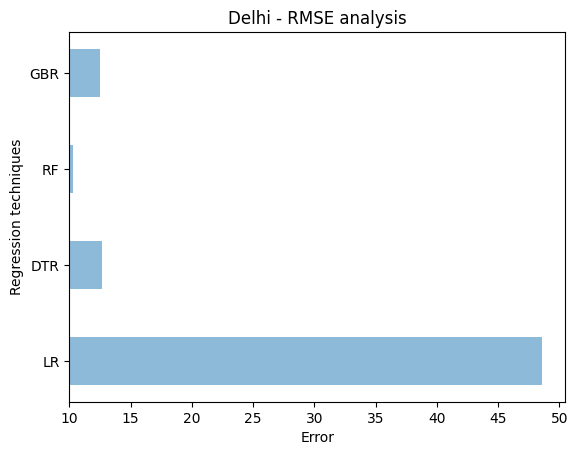
\includegraphics[width=300]{delhi.png}
    \label{fig:Caption}
    \end{figure}
\\ \\
\newpage
\item \textbf{Maharashtra}:  \\ 
        Maharashtra state is also reported to have the highest values of pollution levels in India. We have applied the afore-mentioned regression techniques on Delhi city data set and predicted the values of air quality index in the city and compared it with the actual values. Predicted analysis for Gradient Boosting Regression (GBR), Decision Tree Regression (DTR), Linear Regression (LR) and Random Forest Regression (RFR) is conducted. As seen from the bar graph below, Random Forest Regression technique performs best among all the techniques yielding very low RMSE error. Clearly, its evident that Linear Regression performs worst among all the techniques as it produces very high RMSE error. Decision Tree and Gradient boosting regression techniques performs fairly equivalent yielding same RMSE error.  \\ 
     \begin{figure}[H]
\centering
    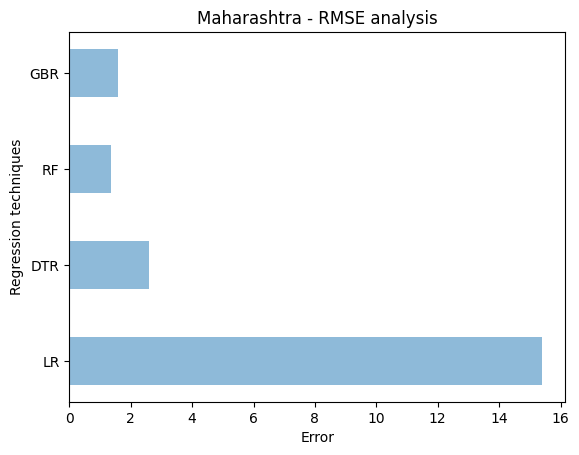
\includegraphics[width=300]{mumbai.png}
    \label{fig:Caption}
    \end{figure}
    \newpage
\item \textbf{Gujarat}: \\
     Gujarat State has fairly low amounts of pollution as compared to Delhi and Maharashtra states. Predicted analysis for Gradient Boosting Regression (GBR), Decision Tree Regression (DTR), Linear Regression (LR) and Random Forest Regression (RFR) is conducted and analyzed. As it is evident that, Decision tree performs best among all the regression techniques. Random Forest and Decision Tree techniques are able to discover more complex dependencies at the cost of more time for fitting, and can handle messier data efficiently, which is why they usually outperform LR models. Similar to above cases, Linear Regression performs worst among all the regression techniques mentioned. \\
     \begin{figure}[H]
     \centering
    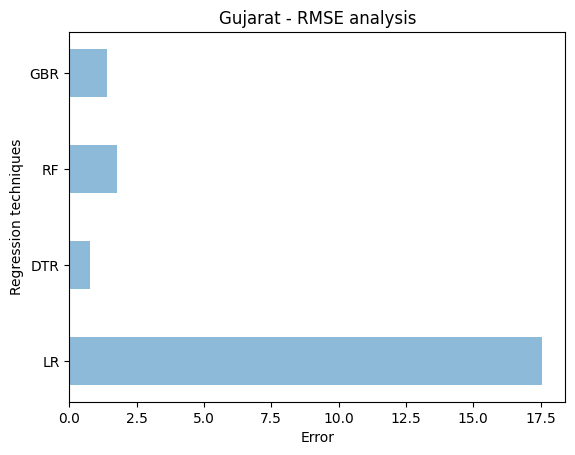
\includegraphics[width=300]{gujarat.png}
    \label{fig:Caption}
    \end{figure}
\\ \\
\end{itemize}
\newpage
\section {Machine Learning Concepts Used}
\\ \\

\subsection {\color{blue}
\textbf{LINEAR REGRESSION}} \\ 
 Linear regression is useful for finding relationship between two continuous variables. One is predictor or independent variable and other is response or dependent variable. It looks for statistical relationship but not deterministic relationship. The core idea is to obtain a line that best fits the data. The best fit line is the one for which total prediction error (all data points) are as small as possible. In this section, we model a probabilistic approach and explicitly model noise using a likelihood estimation. Thereafter, we find the optimal parameters $\theta$ of the model  using techniques like Maximum Likelihood Estimation and Maximum A Posteriori Estimation and analyze the ways to reduce the overfitting present in the model. \\ 

\subsubsection {\color{brown}
\textbf{Mathematical Analysis}} \\ 
\begin{itemize}
    \item 
  \textbf{Maximum Likelihood Estimation} \\
    Linear regression can be applied to our model in order to predict the AQI given the independent variables (pollutants) such as NO2, SO2, RSPM, and SPM.  
    \begin{equation*}
    y = \theta_{0} + \theta_{1}x_{1} + \theta_{2}x_{2} + \theta_{3}x_{3} + \theta_{4}x_{4} 
    \end{equation*}
    where $x_{1}$ = concentration of pollutant $SO_{2}$ \\
    $x_{2}$ = concentration of pollutant $NO_{2}$ \\
    $x_{3}$ = concentration of pollutant $RSPM$ \\
    $x_{4}$ = concentration of pollutant $SPM$ \\
    
    We start with Maximum likelihood equation of the parameters $\theta$. In order to find that, we find $\theta_{ML}$ that maximizes the likelihood function given below: 
    
    \begin{equation*}
    P(Y | X, \theta) = \prod_{n=1}^{N} P(y_{n} | x_{n}, \theta)
    \end{equation*}
    
    Taking the negative likelihood of the above function, we get, 
    
    \begin{equation*}
    L(\theta) = -log(P(Y | X, \theta)) = -log(\prod_{n=1}^{N} P(y_{n} | x_{n}, \theta))
    \end{equation*}
    
    \begin{equation*}
    L(\theta) = -\sum_{n=1}^{N} log( P(y_{n} | x_{n}, \theta))
    \end{equation*}
    
    Let Y = $X^T.\theta$ + $\eta$
    
     \begin{equation*}
    L(\theta) = -\sum_{n=1}^{N} log( P(y_{n} | x_{n}^T \theta, \sigma^2))  = --\sum_{n=1}^{N}  log ( \cfrac{1}{\sqrt{2\pi\sigma^2}} \exp^{\cfrac{-(y_n - x_n^T\theta)^2}{2\sigma^2}})
    \end{equation*}
    
     \begin{equation*}
    L(\theta) = \cfrac{1}{2\sigma^2} - (y_n-x_n^T\theta)^2  + Constant
    \end{equation*}
    
     \begin{equation*}
    L(\theta) = \cfrac{1}{2\sigma^2}(Y - X\theta).^T (Y - X\theta) 
    \end{equation*}
    
    differentiating the negative log likelihood equation wrt $\theta$ and equating it to zero, \\
    \begin{equation*}
    \cfrac{d(L(\theta))}{d\theta} = \cfrac{d}{d\theta}
     [\cfrac{1}{2\sigma^2}(Y - X\theta).^T (Y - X\theta)] = 0 
    \end{equation*}
    
    Solving this, we get 
    \begin{equation*}
    \theta_{ML} = (X^{T}X)^{-1}X^{T}y
    \end{equation*}
    
    where X belongs to $R^{NXD}$ and y belongs to $R^{N}$ \\ 
    
    We performed the same above analysis considering the intercept term in $\theta$ and found out that 
    \begin{equation*}
    RMSE_{intercept} < RMSE_{without\_intercept}
    \end{equation*}
    
\item \textbf{Polynomial Regression} : \\
    The corresponding linear regression model for polynomial regression is: 
    \begin{equation*}
    y = \phi(x)^{T} \theta
    \end{equation*} 
    
    where $\phi(x)$ is a nonlinear feature transformation of the input example x such that 
    \begin{equation*}
     \phi(x) = \begin{bmatrix} x^{0} & x^{1} & x^{2} ... & x^{K} \end{bmatrix}^{T}. 
     \end{equation*} 
     
     On applying the $\Phi$ matrix as mentioned below: 
     \begin{equation*}
    \Phi = \begin{bmatrix} \phi_{0}(x_1) & \phi_{1}(x_1) & .... & \phi_{K-1}(x_1) \\ \phi_{0}(x_2) & \phi_{1}(x_2) & .... & \phi_{K-1}(x_2) \\ ... \\ \phi_{0}(x_N) & \phi_{1}(x_N) & .... & \phi_{K-1}(x_N)  \end{bmatrix}   
     \end{equation*} 
    We get the following equation,
   \begin{equation*}
    y = \theta_{0} + \theta_{1}(x_{1} + x_{2} + x_{3} + x_{4}) + \theta_{2}(x_{1}^{2} + x_{2}^{2} + x_{3}^{2} + x_{4}^{2}) + ..... 
    \end{equation*}
    
    and $\theta_{ML}$ becomes 
   \begin{equation*}
    \bold{\theta_{ML}} = (\Phi^{T}\Phi)^{-1}\Phi^{T}\textbf{y}
    \end{equation*} 
    
    where, $\Phi$ is of the order $R^{N x (k+1)}$ 
    and example \textbf{x} is a D x 1 vector \\
    We calculate $\theta_{ML}$ from the above equation by taking $X_{train}$ into consideration and then, predict $y_{pred}$ values using $X_{test}$ and $\theta_{ML}$.  We calculate RMSE errors of training and testing set on a range of degree of polynomials and observer that as degree of polynomial increases, the RMSE error for testing increases whereas, RMSE error for training decreases, leading to overfit the model. \\  
    
\item \textbf{Maximum A Posteriori Estimation} : \\ 
    The previous observation says that maximum likelihood estimation is prone to overfitting. We often observe that the magnitude of the parameter values becomes relatively large if we run into overfitting. To mitigate the effect of huge parameter values, we can place a prior
distribution on the parameters. 

The posterior over the parameters $\theta$, given the training data X, Y, is obtained by applying Bayes’ theorem as, 
\begin{equation*}
    p(\theta | X, Y) = \frac{p(Y | X, \theta) p(\theta)}{p(Y | X)}
\end{equation*} 

We define the negative log likelihood function and minimize the function to compute the optimal parameters $\theta$ by the following formula,

   \begin{equation*}
    \bold{\theta_{MAP}} = (\Phi^{T}\Phi + (\sigma^2/b^2) I)^{-1}\Phi^{T}\textbf{y}
    \end{equation*}
    
\item \textbf{Regularization} :
    Further, we perform regularization on the model and plot the RMSE error with respect to change in the hyperparameter value - regularization parameter. We observe, as the hyperparameter increases, the RMSE error decreases. For that, $\theta_{ML}$ becomes \\
     \begin{equation*}
    \bold{\theta_{ML}} = (\Phi^{T}\Phi + \lambda I)^{-1}\Phi^{T}\textbf{y}
    \end{equation*}
    
    where $\lambda$ = hyperparameter - regularization parameter to help prevent overfitting of the model.

\subsubsection {\color{brown}
\textbf{Implementation}} 
We define the input matrix as the feature vectors of all the pollutants indexes present in the dataset namely $SO_2$, $NO_2$, $RSPM$, and $SPM$. The output is the air quality index $AQI$ which is calculated by the EPA method in the data pre processing step. The dimensions of input matrix $X$ was (435742, 4) and output label was (435742, 1). Further, we divide this dataset into 80\% training and 20\% testing set. We trained the model and find out parameters using MLE and MAP technique and compared the accuracy of both the methods. Further, to increase the efficiency, we trained our model to find the optimal parameters using polynomial regression and analyzed the nature of the training and testing error with the increase in the degree of polynomial.
\textbf{Simulation parameters:} Training set- 80\% of the whole dataset and testing set- 20\% of the total dataset. \\

\newpage
\subsubsection {\color{brown}
\textbf{Pseudocode}}
\begin{algorithm}
            \caption{Linear Regression (MLE)}
            \begin{algorithmic}
            
                \STATE y is Nx1 vector, X is data(Nxd)
                \STATE $\theta \longleftarrow$ MLE(X,y) 
                \STATE prediction $\longleftarrow$ Xtest * $\theta$
                \STATE Mean Square error $\longleftarrow$ MSE(ytest, prediction)
                
            \end{algorithmic}
        \end{algorithm}
    \begin{algorithm}
            \caption{Maximum Likelihood Estimation- MLE(X, y)}
            \begin{algorithmic}
                \STATE Input: X is NxD data matrix, y is Nx1 vector of dependent variable \\ where N is the total number of samples and D are the features
                \STATE X$\_aug$ $\longleftarrow$ Augmenting extra column of ones on X 
                \STATE P $\longleftarrow$ $X_{aug}^TX_{aug}$
                \STATE Q $\longleftarrow$ $P^{-1}.X\_aug$
                \STATE $\theta$ $\longleftarrow$ Q.y \\
                \STATE Output: $\theta$ (parameters of the model)
            \end{algorithmic}
        \end{algorithm}
        
    \begin{algorithm}
            \caption{Maximum A Posteriori- MAP($X$, y, $\sigma$, $\alpha$)}
            \begin{algorithmic}
                \STATE Input: X is NxD data matrix, y is Nx1 vector of dependent variable \\ where N is the total number of samples and D are the features
                \STATE k $\longleftarrow$ $\frac{\sigma^{2}}{\alpha^{2}}$
                \STATE P $\longleftarrow$ $X^TX$
                \STATE k1 $\longleftarrow$  $P^{-1}$ + $k*I_D$
                \STATE k2 $\longleftarrow$  $X^Ty$  
                \STATE $\theta$ $\longleftarrow$ $k1.k2$
                \STATE Output: $\theta$ (parameters of the model)
            \end{algorithmic}
        \end{algorithm}
        
    \begin{algorithm}
            \caption{Polynomial Regression($X$, k)}
            \begin{algorithmic}
                \STATE Input: X is NxD data matrix, y is Nx1 dependent vector, k is degree of polynomial \\ where N is the total number of samples and D are the features \\
                \STATE Split X and y into X\_train, X\_test, y\_train, y\_test 
                \STATE X$\_aug$ $\longleftarrow$ Augmenting an extra column of ones on X\_train \\
                \STATE X$\_aug\_test$ $\longleftarrow$ Augmenting an extra column of ones on X\_test \\
                \FOR{i=0 to k+1}
                    \FOR{j=0 to N}
                    \STATE ans $\longleftarrow$ 0
                        \FOR{m=0 to D+1}
                            \STATE ans $\longleftarrow$ ans + $X\_{aug}[i][m]^i$ 
                        \ENDFOR
                        \STATE $B[j][i] \longleftarrow ans$
                    \ENDFOR
                \ENDFOR
                \STATE $\theta \longleftarrow MLE\_nonlinear(B,y)$ \\
                \STATE y$\_$pred $\longleftarrow$ \theta.X\_aug\_test   \\
                \STATE Computing RMSE between y\_pred, and y\_test for every value of k (degree of polynomial)
                
            \end{algorithmic}
        \end{algorithm}    
        
   
\newpage
\newpage
 \subsubsection \newpage \textbf{4.1.4} {\color{brown}
\textbf{Results and Inferences}} \\ 
\begin{itemize}
          \item  \textbf{Predicted and Actual AQI values with respect to year} \\ 
       Below is the figure that depicts two plots that indicate predicted AQI values and actual AQI values ith respect to each year present in the dataset. This model was trained and optimal parameters were found using MLE estimation. Then, using this optimal parameters, output label (AQI) was predicted from the input matrix and plotted against each year. This graph represents the amount of error between the actual and predicted values of the output label.
 \\ \\
        \begin{figure}[H]
        \centering
  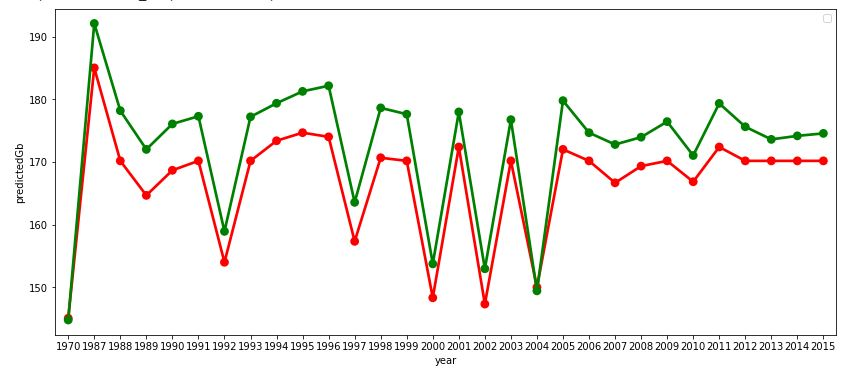
\includegraphics[width=500]{linear_reg_aqi.JPG}
    \caption{Actual and Predicted values against year}
    \label{fig:Caption}
    \end{figure}
   \newpage
      \item  \textbf{Training and Testing RMSE error plotted against the degree of polynomial} \\ 
       Below is the figure that depicts nature of training and testing RMSE (Root Mean Square error) with respect to degree of polynomial in polynomial regression. We observe that training error decreases with an increase in the degree of polynomial whereas, testing error first decreases and then rises as the degree of polynomial increases. It can be inferred that that due to rise in the degree of polynomial, the model tends to overfit and hence, it works well on the training set but not on the unseen data i.e. the test set. Overfitting can be reduced by the use of MAP Estimation or Regularization. \\ \\
        \begin{figure}[H]
        \centering
  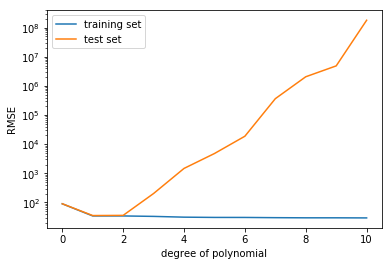
\includegraphics[width=300]{output_33_1.png}
    \caption{RMSE v/s degree of polynomial}
    \label{fig:Caption}
    \end{figure}
    
 \newpage
   \item \textbf{RMSE testing error against the regularization parameter lambda } \\
     Below is the figure that plots testing error RMSE with respect to lambda (regularization parameter). It is used to reduce overfitting by penalizing the parameter values by forcing them close to the origin. Hence, it is evident that as lambda increases, overfitting is prevented and due to this, the testing error decreases with the increasing lambda. \\ \\
     \begin{figure}[H]
     \centering
    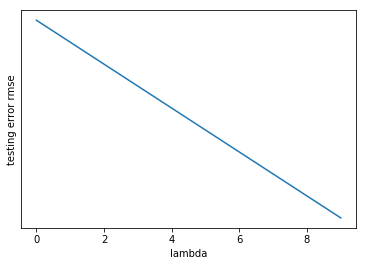
\includegraphics[width=300]{lambda.png}
    \caption{RMSE V/S Lambda(regularization parameter)}
    \label{fig:Caption}
    \end{figure}
\end{itemize}

\end{itemize}

\newpage

\subsection {\color{blue}
\textbf{PRINCIPAL COMPONENT ANALYSIS}} \\ \\
Dimensionality reduction is a method which helps us reduce our computation time by compressing the data-set without losing any useful information. This technique is highly used when there are more than  hundreds or thousands of measurements for each data sample which often leads to failure of statistical models as well. Original Data often contains many redundant, and unimportant features that when removed improves the speed and efficiency of processing and as well as allow us to work with more compact representation of data without losing any vital information. PCA (Principal Component analysis) is one such dimensionality reduction technique. Its main aim is to reduce the dimensionality of a dataset consisting of multiple variables which are correlated with each other and at the same time, retaining maximum variability in the dataset.  It is widely used in applications like facial recognition, computer vision and image compression pertaining to the field of finance, psychology and bioinformatics. This technique transforms the variables/features in the dataset to a set of orthogonal principal components which are also called the eigenvectors of the covariance matrix. They are ordered such that the variable that contributes more variance is listed prior to the variable that contributes less variance comparatively. Hence, the first eigenvector or the first principal component contributes maximum variance. The output generated from PCA are such principal components whose numbers are either lesser or equal to the original variables. 

\subsubsection {\color{brown} \textbf{Mathematical Analysis}}
Given a set of observations x1, x2 , . . . , xn, where each
observation is represented by a vector of length m, the
dataset is thus represented by a window: 

\begin{equation} X_{nm} = 
\begin{bmatrix} 
x_{11} & x_{12} & .... & x_{1m} \\
x_{21} & x_{22} & .... & x_{2m}\\
x_{31} & x_{32} & .... & x_{3m} \\
... & .... & ....    .... \\
x_{n1} & x_{n2} & .......& x_{nm} \\
\end{bmatrix}
\quad
\end{equation}
where X is a m x n matrix with n data samples and m columns/features. In our case, the input matrix consists of about 450000 rows and 4 features corresponding to the pollutant concentrations of $SO_2$, $NO_2$, $RSPM$ and $SPM$. \\
Each data point $x_{n}$ belongs to M dimensional space - $(x_{n1}, x_{n2}, ..., x_{nm})$ \\
Then, we normalize the values by subtracting mean of $X_{nm}$ from it and then further dividing it by the standard deviation: 
      \begin{equation*}
	  \bold{X = (X_{nm} - \mu) / \sigma}
	  \end{equation*}
	  where $\mu$ is the mean of data points in X and $\sigma$ is the standard deviation of feature matrix $X_{nm}$. \\ 
	  
Further, we compute the covariance matrix of the feature matrix $\textbf{X}$, by the following formula \\
 \begin{equation*}
                S = \frac{1}{n}\bold{(X^TX)}
            \end{equation*}
where n is the total number of data points. \\
	  
To apply PCA to transform high dimensional data to low dimension, eigenvalues and corresponding eigenvectors of the covariance matrix S are computed. We choose the K eigenvectors having the largest eigenvalues. Often there will be just a few large eigenvalues, and this implies that k is the inherent dimensionality of the subspace governing the ”signal” while the remaining (m - K) dimensions generally contain noise. We obtain matrix B by stacking the top k eigenvectors corresponding to top k eigenvalues in decreasing order. \\ Further, we calculate the projection matrix, P by the following formula:
   \begin{equation*}
                P = B.B^T
    \end{equation*}

 We know, projected data matrix, $\bar{X}$ can be reconstructed by multiplying the projection matrix with X, 
     \begin{equation*}
                \bar{X} = BB^TX = PX
    \end{equation*}

where B = ($b_1, b_2, b_3, ... , b_K)$ are the top K orthonormal eigen vectors. \\ 
We see, $\bar{X}$ has same dimensions as the original matrix, X but has a significantly lower intrinsic dimensionality as it can be reconstructed from a lower dimensional subspace K. We further take $\bar{X}$ to predict the AQI values and compare with actual AQI values to analyze the data loss and error generated due to dimensionality reduction.  \\

Additionally, to find an K-dimensional subspace of RD that retains as much information as possible, PCA tells us to choose the columns of the matrix B in as the M eigenvectors of the data covariance matrix S that are associated with the M largest eigenvalues. The maximum amount of variance PCA can capture with the first K principal components is : 
       
\begin{equation*}
               V_{K} = \sum_{m=1}^{K} \lambda_{m}
\end{equation*}
where $\lambda_{m}$ is the mth eigenvalue of the co-variance matrix S. 
\\ 

\newpage
\subsubsection {\color{brown} \textbf{Implementation}}
At first, the data was pre-processed according to the steps mentioned in data acquisition step. Then we form the input feature matrix $X$ of dimensions (435742 rows, 4 columns). The columns consists of pollutant indexes that helps to calculate the target output label- air quality index. To apply PCA, we first normalize the feature matrix and compute its covariance matrix S. The dimension of S comes out to be (4,4). Further, we calculate the eigenvalues and eigenvectors of this covariance matrix S and sort the eigenvectors corresponding to decreasing value of eigenvalues. B matrix is formed by stacking top M eigenvectors where M is the lower dimensional space to which we want to reduce the dimension. Further, projection matrix is computed which when multiplied to the feature matrix, yields reconstructed feature matrix $\bar{X}$ that is of the same dimension as $X$ but have a property of constructing from a lower dimensional space M. Further, New AQI values are calculated taking input as the reconstructed feature matrix and values of the reconstructed AQI values and actual AQI values are compared. The development was carried out in Python and execution was done in Google Colab. Pandas library was used for data gathering and processing & Matplotlib and seaborn were used to plot different graphs. \\
\textbf{Simulation parameters:} Number of components for lower dimensional space (M) = 2 \\

The below table is a comparison between actual and reconstrucuted AQI values. The reconstructed AQI values were calculated using the new feature matrix of lower dimension as input. The error can be analyzed as the loss of information that happens when we transform our original space to a lower dimensional space. Here, D (number of features) = 4 and as M (dimension of lower dimensional space) = 2. \\
\begin{table}[h!]
  \begin{center}
    \caption{Comparison of Actual & Reconstructed AQI}
    \label{tab:table1}
    \begin{tabular}{l|S|r} % <-- Changed to S here.
      \textbf{Actual AQI} & \textbf{Reconstructed AQI} \\ 
      \hline
      168.84 & 174.69 \\
      166.84 & 171.12 \\
      167.84 & 179.00 \\
      168.84 & 174.69 \\
      169.65 & 171.12 \\
      167.84 & 172.14 \\
      168.84 & 169.46 \\
    \end{tabular}
  \end{center}
\end{table}


\\ \\

\newpage
\subsubsection {\color{brown} \textbf{PseudoCode}}
\begin{algorithm}
            \caption{Procedure PCA(X, num$\_$components)}
            \begin{algorithmic}
                \STATE sum $\longleftarrow$ 0
                \STATE $\Bar{X}$ $\longleftarrow$ normalize(X)
                \STATE covariance $\longleftarrow$ $\bar{X}$  $\bar{X}^\intercal$
                \STATE S $\longleftarrow$ covariance
                \STATE eigenvecs, eigenvalues $\longleftarrow$ eig(S)
                \FOR{i=1 to num$\_$components}
                    \STATE B $\longleftarrow$ concatenate(B, eigenvecs(i))
                    \STATE sum $\longleftarrow$ sum + eigenvalues(i)
                \ENDFOR
                \STATE P $\longleftarrow$ $B.B^\intercal$
                \STATE $X\_reconstruct$ $\longleftarrow$ $P.X^\intercal$
                \STATE $X\_reconstruct$ $\longleftarrow$ $X\_reconstruct^\intercal$
            \end{algorithmic}
        \end{algorithm}
\begin{algorithm}
    \caption{Loss and Variance Calculations}
    \begin{algorithmic}
        \STATE declaring loss,reconstructions and variances
        \STATE $\bar{X}$, mu, std $\longleftarrow$ normalize(X)
        \FOR{i=1 to 5}
            \STATE reconst, sum $\longleftarrow$ PCA($\bar{X}$,i)
            \STATE error = mse(reconst, $\bar{X}$)
            \STATE reconst $\longleftarrow$ reconst*std + mu
            \STATE reconstructions.append(reconst)
            \STATE variance$\_$values.append(i,sum)
        \ENDFOR
    \end{algorithmic}
\end{algorithm}
\\ \\

\newpage
\subsubsection {\color{brown} \textbf{Results and Inferences}}
\textbf{ 1. Explained Variance - variance attributed to each of the features} \\ 
       After sorting the eigenpairs, the next question is "how many principal components are we going to choose for our new feature subspace?" A useful measure is the so-called "explained variance," which can be calculated from the eigenvalues. The explained variance tells us how much information (variance) can be attributed to each of the principal components. We can see from the below bar graph that 50\% of the variance is contributed by the first principal component, approximately 25\% of the variance is contributed by the second principal component and the rest 2 principal components contributes significantly less than than the first two components. Hence, we choose first two principal components as the low dimensional space. \\ \\
       \begin{figure}[H]
       \centering
     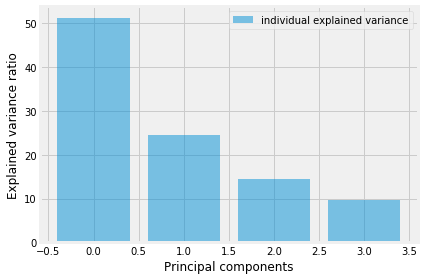
\includegraphics[width=300]{3_variance_ind.png}
    \caption{Explained Variance - variance attributed to each of the features }
    \label{fig:Caption}
\end{figure}
\newpage

    \textbf{ 2. Sorted Eigenvalues in decreasing order} 
    \begin{itemize}
        
       The below graph shows the sorted eigenvalues in decreasing order. We have 4 features, and corresponding to that we have 4 eigenvalues and 4 corresponding eigenvectors found from the covariance matrix S. We sort the eigenvalues in decreasing order and eigenvectors correspondingly. Higher the eigenvalue, higher will be the variance contributed by that eigenvector. \\ 
      \begin{figure}[H]
      \centering
    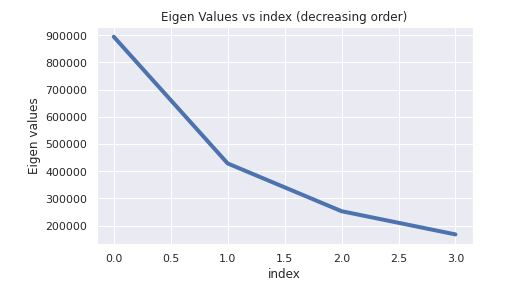
\includegraphics[width=400]{eigenvalues.JPG}
    \caption{ Sorted Eigenvalues in decreasing order  }
    \label{fig:Caption}
    \end{figure}
    \end{itemize}
    
    \newpage
    \textbf{ 3. Maximum Captured Variance  } 
    \begin{itemize}
       
       The below graph shows the maximum amount of variance with respect to the principal components. Maximum captured variance is defined by the sum of the eigenvalues of the principal components taken into consideration. Since, as the x axis represents number of principal components, it means as we go to the right, number of principal components increases and hence, variance would also increase as the number of eigenvalues in the addition is increasing. But Since, eigenvalues are sorted in decreasing order, at first the there is a rapid increase in the captured variance due to high eigenvalues, whereas as we go right, the eigenvalues that are adding have less value, hence it is then increasing though but at a slower rate. \\ \\
   
     \begin{figure}[H]
     \centering
      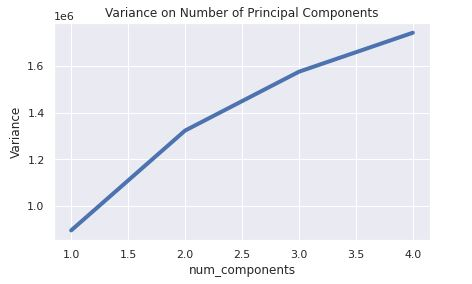
\includegraphics[width=400]{variance.JPG}
    \caption{Maximum Captured Variance }
    \label{fig:Caption}
    \end{figure}

    \end{itemize}
    
   \newpage
    \textbf{ 4. MSE vs number of principal components (sorted eigenvalues) } 
    \begin{itemize}
       
       The below graph shows that the mean squared error with respect to the number of principal components. The reason is that as we take more and more principal components, there is less loss in dimensions and hence, there is less loss in data. Hence, its intuitive that error will decrease as we take more principal components.  \\ \\
        \begin{figure}[H]
        \centering
    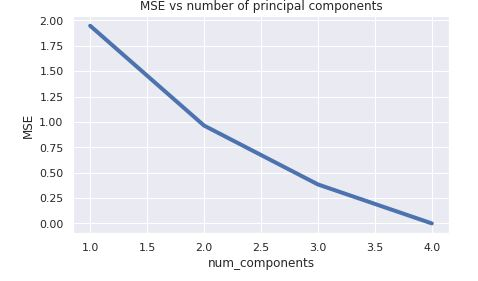
\includegraphics[width=400]{mseerror.JPG}
    \caption{ MSE vs number of principal components (sorted eigenvalues) }
    \label{fig:Caption}
    \end{figure}
    \end{itemize}
\\ \\


\newpage
\subsection {\color{blue}
\textbf{CLASSIFICATION}} \\ \\

\subsubsection {\color{brown} \textbf{Techniques and Models}}
\\ \\
\begin{itemize}
    \item \textbf{Logistic Regression} :
 Logistic regression is a statistical method for predicting binary classes. The outcome or target variable is binary in nature. It is a special case of linear regression where the target variable is categorical in nature. It uses a log of odds as the dependent variable. Logistic Regression predicts the probability of occurrence of a binary event utilizing a logit function. 
 
\item \textbf{Naive Bayes Classification} : It's a probabilistic machine learning model mainly used for classification task. The crux of this classifier is based on the Bayesian theorem. It has a strong assumption of independency between the features. They are robust and easy to implement, however, violations of independence nature of features and problems that are non linearly classfiable poses various problems. 
 
\item \textbf{Support Vector Machines} : It is a supervised machine learning algorithm used for both classification and regression problems. It is based on the idea of finding a optimal hyperplane that best separates the features into different domains. There are three types of kernel available - Linear, Polynomial and Gaussian. A kernel is a way of computing the dot product of two vectors x and y in a very high dimensional feature space.
\end{itemize}

\subsubsection  {\color{brown} \textbf{Mathematical Analysis of Support Vector Machines}} 

Support Vector Machines are based on the idea of finding a hyperplane that best separates the features into different domains. The points closes to the hyperplane are known as the support vectors and the distance between the hyperplane and the points are called the margins. The basic idea is that more faether the support vector points are, from the hyperplane, more is the probability of the points being correctly classified in their corresponding classes. They are importnat in determining the hyperplane as if the support vectors are altered, the position of the hyperplane will change. Hence, hyperplane is also called as margin maximizing hyperplane. \\

The equation of the hyperplane in the ‘M’ dimension can be given as, \\
\begin{equation*}
               y = w_0 + w_1.x_1 + w_2.x_2 + ... 
                 = w_0 + \sum_{i=1}^{m} w_i.x_i  
\end{equation*}

\begin{equation*}
               y  = b + W^T.X
\end{equation*} 

We evaluate that for any point Xi, \\

if $Y_i.(W^T.X_i +b) \geq 1:$ then $X_i$ is correctly classified, else $X_i$ is incorrectly classified. \\ 

So we can see that if the points are linearly separable then only our hyperplane is able to distinguish between them. So these type of SVM is called as hard margin SVM. \\ 

\textbf{Soft Margin SVM}: The data points are not always linearly seperable, hence new slack variable is introduced to overcome the above problem. 
The new equation with the new slack variable $\zeta_{i}$ is, 

\begin{equation*}
               Y_i.(W^T.X_i +b) \geq 1 - \zeta_{i}
\end{equation*} 

if $\zeta_i= 0$, the points can be considered as correctly classified.
else if $\zeta_i> 0$, the points are incorrectly classified.  So if $\zeta_i> 0$, it means that $X_i$ lies in incorrect dimension, thus we can think of $\zeta_i$ as an error term associated with $X_i$. The average error can be given as:
\begin{equation*}
             Error =  \cfrac{1}{n} \sum_{i=1}^{n} \zeta_{i}
\end{equation*}

Hence, The main objective can be stated as, 
\begin{equation*}
              \begin{mini}|l|
        	  {w,b}{\cfrac{1}{2}.W.W  + \sum_{i=1}^{n}\zeta_{i}}{}{}
        	  \addConstraint{Y_i.(W^T.X_i +b) \geq 1 - \zeta_{i}}{}
             \end{mini}
\end{equation*} 

\textbf{Dual from SVM}: When the data points are not linearly seperable, we can separate each data point by projecting it into the higher dimension by adding relevant features to it. The alternative method is dual form of SVM which uses Lagrange’s multiplier to solve the constraints optimization problem whose objective function turns out to be, 
\begin{equation*}
              \begin{maxi}|l|
        	  {w,b}{\sum_{i=1}^{n}\alpha_i - \cfrac{1}{2} \sum_{i=1}^{n} \sum_{j=1}^{n} \alpha_i \alpha_j y_i y_j  (X_i^T.X_j)}{}{}
        	  \addConstraint{\alpha_i \geq 0}{}
        	  \addConstraint{\sum_{i=1}^{n}\alpha_i y_i = 0}{}
             \end{maxi}
\end{equation*}
If $\alpha_i$ $\geq$ 0 then Xi is a Support vector and when αi=0 then Xi is not a support vector. 
A kernel in SVM is a way of computing the dot product of two vectors x and y in a very high dimensional feature space.  \\
The new objective function with kernel function K is, \\
\begin{equation*}
              \begin{maxi}|l|
        	  {w,b}{\sum_{i=1}^{n}\alpha_i - \cfrac{1}{2} \sum_{i=1}^{n} \sum_{j=1}^{n} \alpha_i \alpha_j y_i y_j  K(X_i^T.X_j)}{}{}
        	  \addConstraint{\alpha_i \geq 0}{}
        	  \addConstraint{\sum_{i=1}^{n}\alpha_i y_i = 0}{}
             \end{maxi}
\end{equation*}
\begin{itemize}
The 3 different types of kernels are - linear kernel, polynomial kernel and gaussian kernel. \\
\item \textbf{Polynomial Kernel}: \\
The polynomial kernel is defined as,
\begin{equation*}
        K(X_1, X_2) = (a + X_1^T X_2)^b      
\end{equation*}

\item \textbf{Gaussian Kernel}: \\
The Gaussian kernel is defined as,
\begin{equation*}
        K(X_1, X_2) = \exp^{(-\gamma ||X_1 - X_2||^2)}      
\end{equation*}

\item \textbf{Linear Kernel}: \\
The Linear kernel is defined as,\\
\begin{equation*}
        K(X_1, X_2) = X_1^T X_2     
\end{equation*}
\end{itemize}

\subsubsection  {\color{brown} \textbf{Implementation}} 
In the data pre-processing step, output labels such as $AQI\_Binary\_Range$ and $AQI\_label$ were created. $AQI\_Binary\_Range$ is a binary variable that takes values 0 or 1 based on the value of $AQI$, and $AQI\_label$ is divided into 5 different categories namely - good, moderate, bad, unhealthy, etc that shows the intensity of the pollution in the air. We take the input matrix that includes pollutant concentrations namely $SO_2$, $NO_2$, $RSPM$, and $SPM$ and their $AQI$ indexes. The output label is $AQI\_Binary\_Range$ that is either 0 or 1 (depending on the continuous value of $AQI$ column). This dataset consisting of input features and output label is divided into 80\% training and 20\% test set. Further, the above classification algorithms were applied and analysis was done based on various evaluation metrics that include precision, recall, f1-score and accuracy score. The models were implmented using sklearn library. The development was carried out in Python and was executed in Google Colab. \\
\textbf{Simulation parameters:} Training set- 80\% of the whole dataset and testing set- 20\% of the total dataset, value of C = 100 and $\gamma$ = 0.01 (parameters for polynomial and gaussian kernel) \\

\subsubsection  {\color{brown} \textbf{Evaluation Criteria} }

\begin{itemize}
    \item \textbf{Precision:} Precision is defined by dividing the number of True positives by the Total predictive positives. It talks about how precise/accurate your model is out of those predicted positive, how many of them are actual positive. It is computed by the formula:  \\

\begin{equation*}
               Precision = \frac{True Positive}{True positive + False Positive}
\end{equation*}

\item \textbf{Recall:} Recall is defined by dividing True Positive by Total Actual Positive. It actually calculates how many of the Actual Positives our model capture through labeling it as Positive (True Positive). It is computed by the formula :
\begin{equation*}
               Recall = \frac{True Positive}{True positive + False Negatives}
\end{equation*}

\item \textbf{F1-score/Accuracy Score :} 
\begin{equation*}
               Recall = \frac{2*Precision*Recall}{Precision + Recall}
\end{equation*} 

\item \textbf{Confusion Matrix for Binary classes:} A confusion matrix is a table that is usually used to describe the performance of a classification model on a set of test data whose actual values are already known. It allows the visualization and provides the measurement of the performance of an algorithm. The values of precision and recall are derived from the confusion matrix.

\newcommand\MyBox[2]{
  \fbox{\lower0.75cm
    \vbox to 1.7cm{\vfil
      \hbox to 1.7cm{\hfil\parbox{1.4cm}{#1\\#2}\hfil}
      \vfil}%
  }%
}

\renewcommand\arraystretch{1.5}
\setlength\tabcolsep{0pt}
\hspace{3cm} \begin{tabular}{c >{\bfseries}r @{\hspace{0.7em}}c @{\hspace{0.4em}}c @{\hspace{0.7em}}l}
  \multirow{10}{*}{\rotatebox{90}{\parbox{1.1cm}{\bfseries\centering actual\\ value}}} & 
    & \multicolumn{2}{c}{\bfseries Prediction outcome} & \\
  & & \bfseries 1 & \bfseries 0 \\
  & 1 & \MyBox{True}{Positive} & \MyBox{False}{Negative}  \\[2.4em]
  & 0 & \MyBox{False}{Positive} & \MyBox{True}{Negative} \\
\end{tabular}
\\ \\
\end{itemize}

\subsubsection  {\color{brown} \textbf{Results and Analysis} } 
\begin{itemize}


After processing the above models on the dataset consisting of input features (pollutant concentrations) and binary output label (AQI Binary Range), each model outputs different values of precision and recall. The confusion matrix of each of the algorithms provides a fair way of analyzing these metrics. Precision refers to the percentage of your results which are relevant, recall refers to the percentage of total relevant results correctly classified by your algorithm. Ideal precision and recall value is 1.0, however it is not possible to maximise both hence we evaluate the accuracy (f1 score) which is computed on the basis of precision and recall. \\ \\
\end{itemize}

\begin{itemize}
    \item \textbf{Logistic Regression}: The confusion matrix helps in finding the value of precision and recall. Precision score for this model comes out to be - 0.99 and recall score of 0.99. That accounts for very high accuracy of 0.99.  

\begin{center}
\begin{tabular}{l|l|c|c|c}
\multicolumn{2}{c}{}&\multicolumn{2}{c}{Predicted Outcome}&\\
\cline{3-4}
\multicolumn{2}{c|}{}&Positive&Negative&\multicolumn{1}{c}{}\\
\cline{2-4}
\multirow{2}{*}{Actual Value}& Positive & $81836$ & $72$\\
\cline{2-4}
& Negative & $567$ & $26461$\\
\cline{2-4}
\multicolumn{1}{c}{} & \multicolumn{1}{c}{Total} & \multicolumn{1}{c}{} & \multicolumn{    1}{c}{} & \multicolumn{1}{c}{}\\
\end{tabular} \\ \\
\end{center}
\item \textbf{Naive Bayes Classification}: The confusion matrix helps in finding the value of precision and recall. Precision score for this model comes out to be - 0.96 and recall score of 0.94. This accounts for accuracy of 0.92.  
\begin{center}
\begin{tabular}{l|l|c|c|c}
\multicolumn{2}{c}{}&\multicolumn{2}{c}{Predicted Outcome}&\\
\cline{3-4}
\multicolumn{2}{c|}{}&Positive&Negative&\multicolumn{1}{c}{}\\
\cline{2-4}
\multirow{2}{*}{Actual Value}& Positive & $76061$ & $5307$\\
\cline{2-4}
& Negative & $3123$ & $23905$\\
\cline{2-4}
\multicolumn{1}{c}{} & \multicolumn{1}{c}{Total} & \multicolumn{1}{c}{} & \multicolumn{    1}{c}{} & \multicolumn{1}{c}{}\\
\end{tabular} \\ \\
\end{center}

\item \textbf{Support Vector Machines - Linear Classifier} : The learning of the hyperplane in linear SVM is done by transforming the problem using some linear algebra. For the evaluation of the performance, we find precision and recall from the confusion matrix. Precision score for this model comes out to be - 0.99 and recall score of 0.99. This accounts for accuracy of 0.99. \\
\begin{center}
\begin{tabular}{l|l|c|c|c}
\multicolumn{2}{c}{}&\multicolumn{2}{c}{Predicted Outcome}&\\
\cline{3-4}
\multicolumn{2}{c|}{}&Positive&Negative&\multicolumn{1}{c}{}\\
\cline{2-4}
\multirow{2}{*}{Actual Value}& Positive & $81897$ & $11$\\
\cline{2-4}
& Negative & $475$ & $26553$\\
\cline{2-4}
\multicolumn{1}{c}{} & \multicolumn{1}{c}{Total} & \multicolumn{1}{c}{} & \multicolumn{    1}{c}{} & \multicolumn{1}{c}{}\\
\end{tabular} \\ \\
\end{center}
\newpage
\item \textbf{Support Vector Machines - Polynomial Kernel} : The confusion matrix helps in finding the value of precision and recall. Precision score for this model comes out to be - 0.98 and recall score of 0.98. This accounts for accuracy of 0.98. \\
\begin{center}
\begin{tabular}{l|l|c|c|c}
\multicolumn{2}{c}{}&\multicolumn{2}{c}{Predicted Outcome}&\\
\cline{3-4}
\multicolumn{2}{c|}{}&Positive&Negative&\multicolumn{1}{c}{}\\
\cline{2-4}
\multirow{2}{*}{Actual Value}& Positive & $81811$ & $97$\\
\cline{2-4}
& Negative & $1097$ & $25931$\\
\cline{2-4}
\multicolumn{1}{c}{} & \multicolumn{1}{c}{Total} & \multicolumn{1}{c}{} & \multicolumn{    1}{c}{} & \multicolumn{1}{c}{}\\
\end{tabular}
\end{center}
\\ \\

\item \textbf{Support Vector Machine - Gaussian Kernel} : The confusion matrix helps in finding the value of precision and recall. Precision score for this model comes out to be - 0.998 and recall score of 0.998. This accounts for accuracy of 0.998. \\
\begin{center}
\begin{tabular}{l|l|c|c|c}
\multicolumn{2}{c}{}&\multicolumn{2}{c}{Predicted Outcome}&\\
\cline{3-4}
\multicolumn{2}{c|}{}&Positive&Negative&\multicolumn{1}{c}{}\\
\cline{2-4}
\multirow{2}{*}{Actual Value}& Positive & $81901$ & $7$\\
\cline{2-4}
& Negative & $106$ & $26922$\\
\cline{2-4}
\multicolumn{1}{c}{} & \multicolumn{1}{c}{Total} & \multicolumn{1}{c}{} & \multicolumn{    1}{c}{} & \multicolumn{1}{c}{}\\
\end{tabular} 
\end{center}\\ 
\newpage
\item \textbf{Inference}: \\
The accuracy scores of all the above 5 models were compared. We infer from the below bar graph that Naive Bayes model performs worst among all the applied models still gaining an accuracy of about 92\%. However, other models gain an accuracy of around 98-99\%. The accuracy of the support vector machine models that include polynomial and guassian kernels depends on the hyperparameters C and $\gamma$. As value of C increases, the model tends to overfit. Moreover, if the value of C decreases, the model underfits. Similar behavior is seen in case of $\gamma$ parameter. For large datasets, the probable optimal value of C is high and optimal value of $\gamma$ is low. The optimal value in this case - C = 100 and $\gamma$ = 0.01. The biggest difference between the Naive Bayes algorithm and SVM classifiers (that includes non linear kernels) is that Naive Bayes treats the features as independent whereas SVM looks at the interactions between them to a certain degree. Hence, since in our dataset, there are interactions and correlation between features, SVM is better at capturing those, hence better at the classification task yielding more accuracy than Naive Bayes.  

 \textbf{ Accuracy scores of Classification models} 
         \\ \\
        \begin{figure}[H]
        \centering
    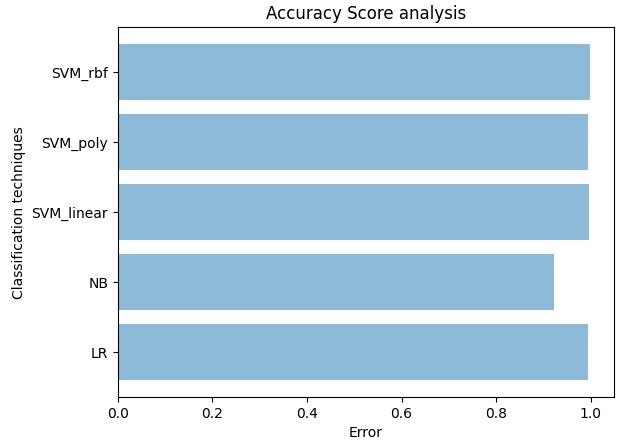
\includegraphics[width=400]{svm.JPG}
    \caption{ MSE vs number of principal components (sorted eigenvalues) }
    \label{fig:Caption}
    \end{figure}



\end{itemize}

\newpage


\subsection {\color{blue}
\textbf{GAUSSIAN MIXTURE MODEL}} \\ \\
Gaussian Mixture Model (GMM) is a type of clustering algorithm. The core idea of this algorithm is to model the dataset as a mixture of several Gaussian Distributions. In this case, “Gaussian” means the multivariate normal distribution $\mathcal{N}(\mu, \Sigma)$ and “mixture” means that various different gaussian distributions, all with different mean $\mu_{j}$ and different covariance matrices $\Sigma_{j}$, are combined by taking the weighted sum of the probability density functions. This is called the likelihood function, 

\begin{itemize}

\begin{equation}
   p(\mathbf{x} | \mu, \Sigma, \pi) = \sum^k_{j=1} \pi_j {\mathcal{N}(\mathbf{x} | \boldsymbol{\mu}_j, \Sigma_j)} 
   \end{equation}
   
subject to
\begin{align}
\sum_{j=1}^k \phi_j = 1 
   \end{align}

Moreover, the probability density function of a Gaussian Distribution In one dimension  is given by, 
\begin{align}
\mathcal{N}(\mathbf{x} | \boldsymbol{\mu}, \Sigma) = \cfrac{1}{\sigma \sqrt{2\pi}}  \exp^{-\cfrac{(x-\mu)^2}{2\sigma^2}}
   \end{align}
   
 For Multivariate (example d-variate) Gaussian Distribution, the probability density function is as follows,
 \begin{align}
\mathcal{N}(\mathbf{x} | \boldsymbol{\mu}, \Sigma) = \frac{1}{\sqrt{(2\pi)^k |\Sigma_j|}} \text{exp}\Bigg( 
    - \frac{(\mathbf{X}_i - \boldsymbol{\mu}_j)^T \Sigma_j^{-1} (\mathbf{X}_i - \boldsymbol{\mu}_j) }
         {2} 
  \Bigg)
   \end{align} 

Since, the parameters cannot be estimated in closed form. This is where Expectation-Maximization algorithm is beneficial. The Expectation-Maximization (EM) algorithm is an iterative way to find maximum-likelihood estimates for model parameters when the data is incomplete or has some missing data points or has some hidden variables.  \\ \\

E - step: \\

The responsibility for each data point x is defined as, \\
\begin{align}
\gamma_{k}(x) =  \frac{ P(x|k) \pi_{k} }{ \sum_{k=1}^K P(x|k) \pi_{k} } 
\end{align}


M-step: \\
Now for the log likelihood function to be maximum, its derivative of $p(X|\mu, \Sigma, \pi)$ with respect to  $\mu$, $\Sigma$ and $\pi$ should be zero. \\

So equaling the derivative of  $p(X|\mu, \Sigma, \pi)$ with respect to $\mu$ to zero and rearranging the terms, we get, \\

\begin{align}
\boldsymbol{\mu}_k = {1 \over {n}}\cfrac{\sum_{n=1}^N \gamma_{k}(x_n) x_{n}}{\sum_{n=1}^N \gamma_{k}(x_n)} 
\end{align}
\\

Equaling the derivative of  $p(X|\mu, \Sigma, \pi)$ with respect to $\Sigma$ to zero and rearranging the terms, we get, \\

\begin{align}
\boldsymbol{\Sigma}_k = {1 \over {n}}\cfrac{\sum_{n=1}^N \gamma_{k}(x_n) (x_{n} - \gamma_{k})(x_{n} - \gamma_{k})^T}{\sum_{n=1}^N \gamma_{k}(x_n)} 
\end{align}
\\

Equaling the derivative of  $p(X|\mu, \Sigma, \pi)$ with respect to $\pi$ to zero and rearranging the terms, we get, \\

\begin{align}
\boldsymbol{\pi}_k = {1 \over {n}} \sum_{n=1}^N \gamma_{k}(x_n)
\end{align}
\\

 where $\sum_{n=1}^N \gamma_{k}(x_n)$ denotes the total number of sample points in the k-th cluster. \\ \\
\end{itemize}

\subsubsection {\color{brown}
\textbf{Implementation}} \\ 
\begin{itemize}

At first, Dataset is pre-processed and AQI column was calculated based on the different pollutant indexes as mentioned in the data acquisition step. Then input data is formed by stacking any two features (pollutants) such as $SO_2$ and $NO_2$, $SO_2$ and $SPM$ and $NO_2$ and $SPM$. 
Then GMM model was applied that firsts initialized the means, and variances to random values. Further, responsibility matrix was computed using probability density functions of each data point as a part of E step. Further, Means and variances were updated as a part of M-step. After processing the model, we plotted 2 clusters in the form of contours using the final value of means and covariances. These two clusters can be inferred as two groups that have different values of the binary output label - $AQI\_Binary\_Range$ that takes only two values - 0 and 1. The development was carried out in Python and execution was done in Google Colab. Pandas library was used for data reading, gathering and processing. Matplotlib and seaborn were used to plot different graphs.  
\end{itemize}
\newpage

\subsubsection {\color{brown}
\textbf{Psuedocode}} \\ 
\begin{algorithm}

        \caption{algorithm for Gaussian mixture modeling (GMM)}
        \begin{algorithmic}
            \STATE P = Input feature matrix 
            \STATE K = Number of Probability Distribution 
            \STATE $\pi$ = Weight of Probability Distribution 
            \STATE $\mu$ = Mean of Probability Distribution
            \STATE $\Sigma$ = Co-variance of Probability Distribution
            \STATE Input: P and K
            \STATE Parameter Initialization $\pi$, $\mu$ and $\Sigma$
           \FOR{t=1 to T}
                   \FOR{n=1 to  N}                  
                        \FOR{k=1 to K}
                         \hspace{1cm}\gamma(z_{nk})=\cfrac{\pi_kN(p_n|\mu_k,\Sigma_k)}{\sum_{i=1}^{N}\pi_i N(p_n|\mu_i,\sigma_i)}
                    
                        \ENDFOR
                    \ENDFOR
                    \STATE
                    {  \FOR{k=1 to K}
                         \hspace{1cm}\mu_k=\cfrac{\sum_{i=1}^{N}\gamma(z_{nk})p_n}{\sum_{i=1}^{N}\gamma(z_{nk})}
                         \newline
                          .\hspace{1cm}\Sigma_k=\cfrac{\sum_{i=1}^{N}\gamma(z_{nk})(p_n-\mu_k)(p_n-\mu_k)^T}{\sum_{i=1}^{N}\gamma(z_{nk})}
                          \newline
                          .\hspace{1cm}\pi_k=\cfrac{1}{N}\sum_{i=1}^{N}\gamma(z_{nk})
                    
                        \ENDFOR
                    }
                   \ENDFOR
                    \newline
                   Output: \pi, \mu and \Sigma
        \end{algorithmic}
    \end{algorithm}

\newpage
\subsubsection {\color{brown}
\textbf{Results and Inferences}} \\ 

\begin{itemize}
\item \textbf{$SO_2$ vs $NO_2$ clusters (before and after GMM)}

\subfloat{{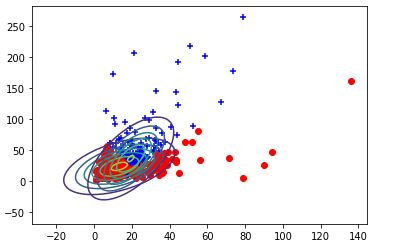
\includegraphics[width=7cm]{1_before_so2_no2.JPG} }}%
    \qquad
\subfloat{{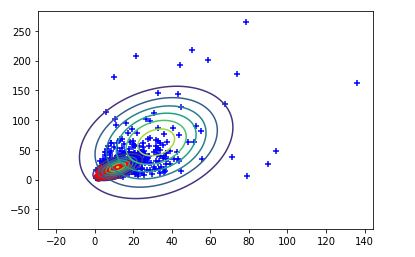
\includegraphics[width=7cm]{2_after_so2_no2.JPG} }}% 
\\ The left graph shows the clusters plotted on the scatter graph $SO_2$ and $NO_2$ before applying the GMM model and the right graph are the new reformed clusters after applying the GMM model. Since, our $AQI_Binary_Range$ takes two binary values - 0 or 1, hence these two clusters corresponds to two different groups of AQI values.  \\ \\
\end{itemize}

\begin{itemize}
\item \textbf{$NO_2$ vs $SPM$ clusters (before and after GMM)}

\subfloat{{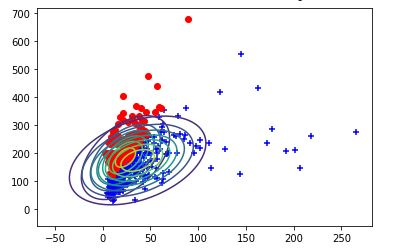
\includegraphics[width=7cm]{3_before_no2_spm.JPG} }}%
    \qquad
\subfloat{{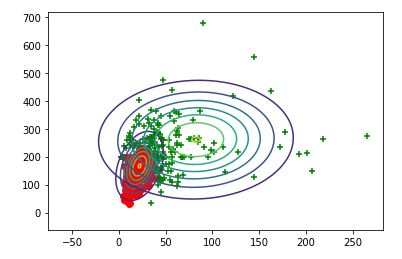
\includegraphics[width=7cm]{4_after_no2_spm.JPG} }}% 
\\ The left graph shows the clusters plotted on the scatter graph $NO_2$ and $SPM$ before applying the GMM model and the right graph are the new reformed clusters after applying the GMM model. Since, our $AQI_Binary_Range$ takes two binary values - 0 or 1, hence these two clusters corresponds to two different groups of AQI values.  \\ \\\newpage
\end{itemize}

\begin{itemize}
\item \textbf{$SO_2$ vs $SPM$ clusters (before and after GMM)}

\subfloat{{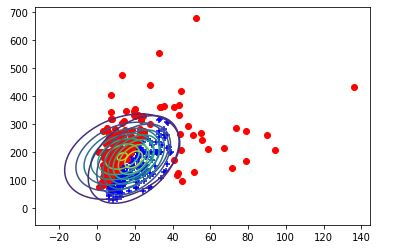
\includegraphics[width=7cm]{5_before_so2_spm.JPG} }}%
    \qquad
\subfloat{{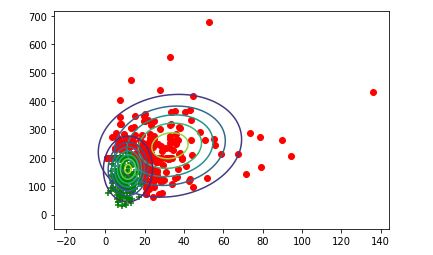
\includegraphics[width=7cm]{6_after_so2_spm.JPG} }}% 
\\ The left graph shows the clusters plotted on the scatter graph $SO_2$ and $SPM$ before applying the GMM model and the right graph are the new reformed clusters after applying the GMM model. Since, our $AQI_Binary_Range$ takes two binary values - 0 or 1, hence these two clusters corresponds to two different groups of AQI values.  \\
\end{itemize}

\section{Conclusions}
\begin{itemize}
	
Our main objective was to apply knowledge of different machine learning concepts to solve a major environmental problem. In this work, we analyzed the air quality dataset that consisted of different pollutant concentrations and other metereological variables of different states and cities of India taken at different time frames. Different techniques like Linear Regression using Maximum Likelihood Estimation and Maximum A Posteriori Estimation, were implemented  in order to predict the air quality index. We inferred that the RMSE error in MAP estimation was less than the RMSE error in the MLE estimation as MAP estimation overcomes the problem of overfitting and hence, reducing the testing error. Furthermore, On applying the Polynomial Regression for multiple features in order to better fit the data, we analyzed that as the degree  of  polynomial  increases,  the  training error  decreases  whereas  testing  error  first  decreases  a  little  and  then  increases. It  is  because  as polynomial degree increases,  model becomes more complex,  thus giving rise to overfitting which fits the training set but does not work well on the unseen data (test set). Furthermore, to reduce the effect of over fitting, we introduced the regularization parameter and observed that with increase of the regularization parameter, the testing error reduces linearly. Furthermore, we applied Dimensionality reduction technique, PCA (Principal Component Analysis) that helps to reduce the dimensions of the data and increase the speed and efficiency of the model without any major loss of information. We plotted the variance of each of the features which is contributed to the data and inferred that as we increase the number of principal components for the lower dimensional space to which we want to reduce, the MSE error decreases as less loss of data is incurred. We applied Classification models such as Support Vector Machines, Logistic Regression and Naive Bayes in order to predict the AQI and analyze the error performance for each of these models. We inferred that Naive Bayes performs works among all the models and Support Vector Machines using Gaussian Kernel performs best yielding the lowest possible RMSE error. We applied Gaussian Mixture Model (GMM) to our data to cluster the data points into two groups with respect to different features (pollutant concentrations) of the dataset. The two clusters are analagous to the two groups of values having $AQI_{label}$ value 0 and 1 indicating Good and Bad air quality conditions.Thus, For future work, we intend to investigate the other factors effecting the air pollution.
\end{itemize} 

\section{ Contribution of team members}	
\subsection{Technical contribution of all team members }
Enlist the technical contribution of members in the table. Redefine the tasks (e.g Task-1 as simulation of fig.1 and so on)
\begin{table}[h]
\centering
\begin{tabular}{|c|c|c|c|c|}
\hline
Tasks  & Muskan & Rushil & Vishal & Mohit \\ \hline
Initial Work &    Choosing Base Article           &         Choosing Base Article       &     Finding Dataset         &      Finding Dataset        \\ \hline
Dataset &  Dataset Preprocessing &   Data Analysis   &    Data Pre processing   & Data Analysis           \\ \hline
Linear Regression & MLE, Poly Regression code  &  Mathematical analysis  &   Mathematical analysis  &    MAP code   \\ \hline
PCA &     PCA code  &  Mathematical analysis  &  Integration    &   Mathematical analysis  \\ \hline
\makecell{Article \\ Reproduction}  &   \makecell{Gradient Boosting \\and final Figures}   &  Random Forest  &  Linear regression    &  Decision Tree  \\ \hline
\makecell{Classification}  &   Coding and  Figures   &  Integration  &  Mathematical analysis   &  Mathematical analysis \\ \hline
\makecell{GMM}  &   \makecell{GMM model code and maths}   & Mathematical analysis  &  GMM clustering   &  Integration \\ \hline

\end{tabular}
\end{table}



\subsection{Non-Technical contribution of all team members }
Enlist the non-technical contribution of members in the table. Redefine the tasks (e.g Task-1 as report writing etc.)
\begin{table}[h]
\centering
\begin{tabular}{|l|l|l|l|l|}
\hline
Tasks  & Muskan & Rushil & Vishal & Mohit \\ \hline
\makecell{Mathematical Analysis \\ handwritten} &   \makecell{ Linear Regression, \\ GMM}            &         PCA       &     GMM        &      Classification        \\ \hline
Final Report &  \makecell{ML concepts used \\ Results and \\ mathematical analysis} &   \makecell{Pseudocodes \\ Motivation \\ and Problem statement}   &    \makecell{Literature Review and \\ Data Acquisition}   & \makecell{Pseudocode and \\ Background, \\ Related Work}           \\ \hline

\end{tabular}
\end{table}

\begin{thebibliography}{9}
\bibitem{ref1} Dominici, F.; Peng, R.D.; Bell, M.L.; Pham, L.; Dermott, A.M.; Zeger, S.L.; Samet, J.M.\\ \textit{Fine particulate air
pollution and hospital admission for cardiovascular and respiratory diseases. J. Am. Med. Assoc. 2006, 295,1127–1134.}

\bibitem{ref2} Li, P.; Xin, J.; Wang, Y.; Wang, S.; Li, G.; Pan, X.; Liu, Z.; Wang, L.\\
\textit{The acute effects of fine particles on
respiratory mortality and morbidity in Beijing, 2004–2009. Environ. Sci. Pollut. Res. Int. 2013, 20, 6433–6444.}

\bibitem{ref3}
Pope, C.A., III; Burnett, R.T.; Thun, M.J.; Calle, E.E.; Krewski, D.; Ito, K.; Thurston, G.D.\\
\textit{Lung cancer,cardiopulmonary mortality, and long-term exposure to fine particulate air pollution. J. Am. Med. Assoc. 2002,287, 1132–1141.}

\bibitem{ref4}
A. Gautam,; M. Mahajan ,; S. Garg (2003)\\
\textit {Impact of air pollution on human health in Dehradoon city.}

\bibitem{ref5}
Herbert Schimmel ,; Thaddeus J. Murawski.(1975)\\
 \textit{SO\textsubscript{2}\textendash Harmful Pollutant or Air Quality Indicator?, Journal of the Air Pollution Control Association, 25:7, 739-740, DOI:
10.1080/00022470.1975.10470136}

\bibitem{ref6}
https://www.kaggle.com/sharmamanali/air-quality-index-analysis-ml-visualisation

\bibitem{ref8}
Athanasiadis, I.N.; Kaburlasos, V.G.; Mitkas, P.A.; Petridis, V. Applying machine learning techniques on air
quality data for real-time decision support. In Proceedings of the First international NAISO Symposium on
Information Technologies in Environmental Engineering (ITEE’2003), Gdansk, Poland, 24–27 June 2003.

\bibitem{ref9}
Kurt, A.; Oktay, A.B. Forecasting air pollutant indicator levels with geographic models 3 days in advance
using neural networks. Expert Syst. Appl.2010, 37, 7986–7992.

\bibitem{ref10}
Dan wei: Predicting air pollution level in a specific city 
[2014]

\bibitem{ref11}
José Juan Carbajal-Hernándezab Luis P.Sánchez-Fernándeza 
Jesús A.Carrasco-OchoabJosé Fco.Martínez-Trinidadb: 
Assessment and prediction of air quality using fuzzy logic 
and autoregressive models: Center of Computer Research –
National Polytechnic Institute, Av. Juan de Dios Bátiz S/N, 
Gustavo A. Madero, Col. Nueva. Industrial Vallejo, 07738 
México D.F., Mexico1. (2012) Doi 
:https://doi.org/10.1016/j.atmosenv.2012.06.004

\bibitem{ref12}
M. Dong, D. Yang, Y. Kuang, D. He, S. Erdal, and D. Kenski, “PM\textsubscript{2.5} concentration prediction using hidden semi-markovmodel-based times series data mining,” Expert Syst. Appl., vol. 36, no. 5, pp. 9046–9055, Jul. 2009.

\bibitem{ref13}
S. Thomas and R. B. Jacko “Model for forecasting expressway pm2.5 concentration \textendash application of regression and neural network models." Journal of the Air \& Waste Management Association, vol. 57, no. 4,pp. 480–488, 2007.

\bibitem{ref14}
Shaban, Khaled Bashir, Abdullah Kadri, and EmanRezk. "Urban air pollution monitoring system with forecasting models." IEEE Sensors Journal 16, no. 8 (2016): 2598-2606.

\bibitem{ref15}
Jain, Varun, MansiGoel, MukulikaMaity, VinayakNaik, and
RamachandranRamjee. "Scalable measurement of air pollution using COTS IoT devices." In Communication Systems \& Networks (COMSNETS), 2018 10th International Conference on, pp. 553-556.IEEE, 2018.

\bibitem{ref16}
MdNazmulHoq, RakibulAlam, Ashraful Amin, “Prediction of
possible asthma attack from air pollutants: towards a high density air pollution map for smart cities to improve living”, International Conference on Electrical, Computer and Communication Engineering (ECCE), 7-9 February, 2019.

\bibitem{ref17}
Aditya C. R.;Chandana R. Deshmukh; Nayana D. K.; Praveen Gandhi Vidyavastu;Associate Professor, Department of Computer Science and Engineering,B.E. Student,Department of Computer Science and Engineering,Vidya Vikas Institute of Engineering and Technology,Mysuru, Karnataka, India 570028.

\bibitem{ref18}
Kalapanidas, Elias & Avouris, Nikolaos. (1999). Applying Machine Learning Techniques in Air Quality Prediction. 

\bibitem{ref19}
O. A. Ghoneim, Doreswamy and B. R. Manjunatha, "Forecasting of ozone concentration in smart city using deep learning," 2017 International Conference on Advances in Computing, Communications and Informatics (ICACCI), Udupi, 2017, pp. 1320-1326. 
\bibitem{ref20}
D. Zhu, C. Cai, T. Yang, and X. Zhou‘‘A machine learning approach for air quality prediction: Model regularization and optimization,’’ Big Data Cogn. Comput., vol. 2, no. 1, p. 5, 2018. 
\bibitem{ref21}
S. Ameer et al., "Comparative Analysis of Machine Learning Techniques for Predicting Air Quality in Smart Cities," in IEEE Access, vol. 7, pp. 128325-128338, 2019.
\bibitem{ref22}
L. Breiman, ‘‘Random forests,’’ Mach. Learn., vol. 45, no. 1, pp. 5–32,2001.

\bibitem{ref23}
C. A. Keller, M. J. Evans, J. N. Kutz, and S. Pawson, \textbackslash Machine Learning and Air Quality Modeling," pp. 4488\{4494, 2017.

\bibitem{ref24}
 A. Ben Ishak, M. Ben Daoud, and A. Trabelsi, \textbackslash Ozone Concentration
Forecasting Using Statistical Learning Approaches," vol. 8, no. 12, pp.
4532\{4543,2017.

\bibitem{ref25}
R. W. Gore, \textbackslash An Approach for Classification of Health Risks Based on
Air Quality Levels," pp. 58\{61, 2017

\bibitem{ref26}
Asgari, Marjan, Mahdi Farnaghi, and Zeinab Ghaemi. "Predictive
mapping of urban air pollution using Apache Spark on a Hadoop
cluster." In Proceedings of the 2017 International Conference on
Cloud and Big Data Computing, pp. 89-93. ACM, 2017

\bibitem{ref27}
C. Yan, S. Xu, Y. Huang, Y. Huang, and Z. Zhang, \textbackslash Two-Phase Neural
Network Model for Pollution Concentrations Forecasting," Proc. - 5th
Int. Conf. Adv. Cloud Big Data, CBD 2017, pp. 385\{390, 2017.
\end{thebibliography}
\end{document} 